\chapter{Wi-Fi-beállítás}
Normál működés közben a Wi-Fi ki van kapcsolva. Beállításkor tartsa a telefont körülbelül 10–20 cm-re a kijelzőtől. Az alapértelmezett jelszó 1234567890, a kezelőfelület címe http://192.168.4.1.

Leválasztott USB mellett kapcsolja be a gyújtást vagy a tápellátást, majd azonnal nyomja meg a hátoldali gombot. A kijelzőn QR-kód jelenik meg. Kapcsolja ki a telefon mobiladat-kapcsolatát, olvassa be a QR-kódot, és csatlakozzon a műszer Wi-Fi-hálózatához. Nyissa meg a kezelőfelületet böngészőben, válassza ki az alkalmazást és a hozzá illő érzékelőt, mentse a beállítást, majd kapcsolja ki és vissza a gyújtást.

Kapcsolódási hiba esetén vigye közelebb a telefont, és ellenőrizze, hogy internetelérés hiányában is a műszer hálózatán marad-e. Szükség esetén ismételje meg a QR-kódos indítást. A hátoldali gomb az alkalmazások kezelésére és az első programozás indítási módjának kiválasztására is szolgál.

Az USB az első programozáshoz használható; a későbbi firmware-frissítéshez a webes felület ajánlott. USB használata előtt válasszon le minden járművezetéket. Kövesse az adott firmware útmutatóját; a forrás nem ismertet helyreállítási eljárást vagy feltöltési menüt.

\begin{figure}[H]
\centering
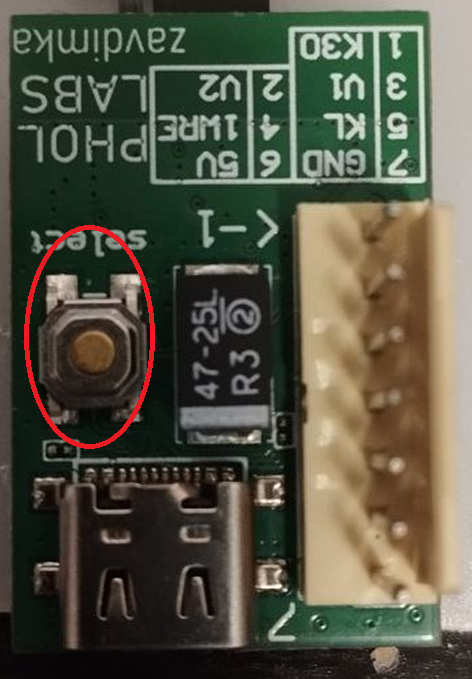
\includegraphics[width=.85\textwidth,height=.60\textheight,keepaspectratio]{figures/ivevo/image11.png}
\caption{Wi-Fi-beállítás}
\end{figure}
